\documentclass{article}

\usepackage{import}
\usepackage{pdfpages}
\usepackage{transparent}
\usepackage{xcolor}
\usepackage{amsmath, amsthm, amsfonts, amsthm, amssymb, mathtools, mathrsfs}
\usepackage{graphicx} 
\usepackage{tikz, tikz-cd} 
\usepackage{hyperref}
\usepackage[shortlabels]{enumitem} 
\usepackage[margin=1in]{geometry} 


\newcommand{\R}{\mathbb{R}}
\newcommand{\Q}{\mathbb{Q}}
\newcommand{\Z}{\mathbb{Z}}

\newcommand{\A}{{\tt Area}} 
\newcommand{\N}{\mathbb{N}}
       %	\newcommand{\incfig}[2][1]{%
%	    \def\svgwidth{#1\columnwidth}
%	    \import{./figures/}{#2.pdf_tex}
%}
%\pdfsuppresswarningpagegroup=1

\newtheorem{prb}{Problem}

\title{MTH 322 Midterm }
\author{Evan Fox} 
\date{10/22}


\begin{document}
\maketitle
	   \begin{prb}  \end{prb} 
	   \begin{proof} 
	   	\begin{enumerate}
	   		\item Squaring the sphere is one of the great unsolved problems in mathematics. 
				The orginal statement of the problem dates back thousands of years
				to acient Greece and it wasn't 
				fully solved until 1882. The problem asks to construct (using ruler and compass) 
				a square, with the same area of a given sphere. It turns out that this is actually 
				impossible, since such a square would have side length $\sqrt{pi}$, which is 
				transendental, and it is not possible to construct transendental numbers since 
				using ruler and compass construction you can only add, subtract, multiply, devide, 
				and take square roots. 


			\item Trisecting an angle using only a compass and straightedge is another problem 
				which also dates back to ancient Greece and went unsolved for thousands 
				of years. It is 
				well known and we did it in class that 
				it is possible to \emph{bisect} and angle, 
				here the challenge to to take an angle $ABC$ and construct two
				lines passing through $B$ such that the three angles created are all congruent, i.e. 
				we want to \emph{trisect} the angle. While it is possible to trisect a line 
				into three congruent segments (as shown in the yt video), it is not 
				possible to trisect an angle since algebraically it involes taking a 
				cube root, which is not possible with ruler and compass alone. The proofs 
				of these results require Galios theory. 

		\end{enumerate}
	   \end{proof}  

	   \begin{prb}  \end{prb} 
	   \begin{proof} 
	   	\begin{enumerate}[(a)]
			\item The volume a Sphere is $S = \frac{4}{3} \pi r^3$ and the volume of a cylinder is 
				$C = \pi r^3$, so the ratio of their volumes is $S/C = 
				\frac{4}{3}$. 

			\item 
				Using notation as in the given picture; note that 
				the triangles $BDE$ and $CED$ will have the same area, 
				first, it is clear that the both have the same base $DE$, then since the distence 
				between parallel lines remains constant 
				(in Euclidian plane), and both triangle have thier 
				enpoints on the parallel lines $DE$ and $BC$, both triangles have the same height. 
				Then since area is given by $\A = \frac{1}{2}bh$ with $b$ the base and $h$ 
				the height, we have $\A(BDE) = \A(CED)$. 

				Now we can also consider the triangle $BDE$ with base $DB$ (as 
				opposed to $DE$ above), and its area can be written as $\A(BDE) = \frac{1}{2}|BD|h$ for
				some $h$, simillarly, $\A(CED) = \frac{1}{2} |CE| h^\prime$. Using the argument of the
				preceeding paragraph, we have $\frac{1}{2}|BD|h = \frac{1}{2} |CE| h^\prime$. 
				We also apply this argument to the triangle $ADE$, that is 
				$\A(ADE) = \frac{1}{2} |AD| h = \frac{1}{2} |AE| h^\prime$. 
				Then 
				\[ \frac{|AD|}{|DB|} = \frac{\tfrac{1}{2}|AD|h}{\tfrac{1}{2}|DB|h} 
				=  \frac{\tfrac{1}{2}|AE|h^\prime}{\tfrac{1}{2}|CE|h^\prime} = \frac{|AE|}{|CE|} \]
				Which gives the result. 
	   	\end{enumerate}	
	   \end{proof} 

	   \begin{prb}  \end{prb} 
	   \begin{proof} 
	   	First, we will find the area of the shaded cross section of the semi-sphere as a function of $h_2$. 
		By the Pythagorean theorem, $r = \sqrt{R^2 - h_2^2} $, so $\A( \text{cross section }) = \pi r^2 
		= \pi(R^2 - h_2^2)$. Now we must find the area of the shaded cross secton of the cylinder with 
		a cone removed in terms of $h$, the area of a cross section of the cylinder is $\pi R^2$ since 
		it has radius $R$ and we are removing a cicle of raduis $\pi h^2$, so the shadded area 
		$\A = \pi R^2 - \pi h^2 = \pi(R^2 - h^2)$. Now the raduis of the semi-cirlce is $R$ and the 
		height of the cylinder is $R$, so since the function for the area of a cross section 
		of the semi-sphere and the area of a cross sectoin of the cynlinder with a cone removed are the same
		and since both $h$ and $h_2$ take values in $[0, R]$, it follows from Cavalieri's principle that 
		the two shapes have the same volumue (There is a one to one corrospondence between cross sections
		by taking the cross section determined hy $h_2$ and mapping it to the one determined by $h$). 
		But the volume of the cylinder with a cone removed is $\pi R^3 - \frac{1}{3}\pi R^3 = \frac{2}{3} \pi R^3$. 
		Then since the semi-sphere has half the volume of a sphere, the volume of a whole sphere is 
		$\frac{4}{3} \pi R^3$
	   \end{proof} 

	   \begin{prb}  \end{prb} 
	   \begin{proof} 
	         Given a quadrilateral $Q$ with sides $a, b, c, d$ (with $a$ and $c$ disjoint), 
		 we can decompose the area of $Q$ into the sum of two triangles in two ways, the first 
		 way by considering the triangles formed after drawing the diagonal from 
		 the point incident to $a$ and $b$ to the one incident with $c$ and $d$. This gives 
		
		 \begin{equation} 
			 \A(Q) = \frac{1}{2}ad \sin(\theta_1) + \frac{1}{2} cd \sin(\theta_2) 
	         \end{equation}

		 We can also decompose the area of $Q$ into the sum of the area of two triangles 
		 by drawing in the diagonal from the point incident to both $a$ and $d$ and the 
		 point incident to both $b$ and $c$, this gives 

		 \begin{equation}
		 	\A(Q) = \frac{1}{2}ab \sin(\theta_3) +\frac{1}{2} cd \sin(\theta_4) 
		 \end{equation}
		
		 Now addint together equations 1 and 2  (and noting that $ 0< \theta_i \leq \frac{\pi}{2}$), we get 
		 \begin{equation}
		 	2\A(Q) = \A(Q) = \frac{1}{2}ad \sin(\theta_1) + \frac{1}{2}cd \sin(\theta_2) +  \frac{1}{2}ab \sin(\theta_3) + \frac{1}{2}cd \sin(\theta_4) \leq \frac{1}{2}(ad + ab + cd + cb) = \frac{1}{2}(a + c)(b+ d) 
		 \end{equation}
	   Note that at the one step where we have an inequality, equality is obtained iff $\sin(\theta_i) = \frac{\pi}{2}$ for $i = 1,2,3,4$, in which case $Q$ has all internal angles equal to 90 degrees, that is to say that $Q$ is 
	   a rectangle. Now 
	   deviding both sides of the last equation by two gives the result. 

	   \end{proof} 

	   \begin{prb}  \end{prb} 
	   \begin{proof} 
	   	\begin{enumerate}[(a)]
			\item 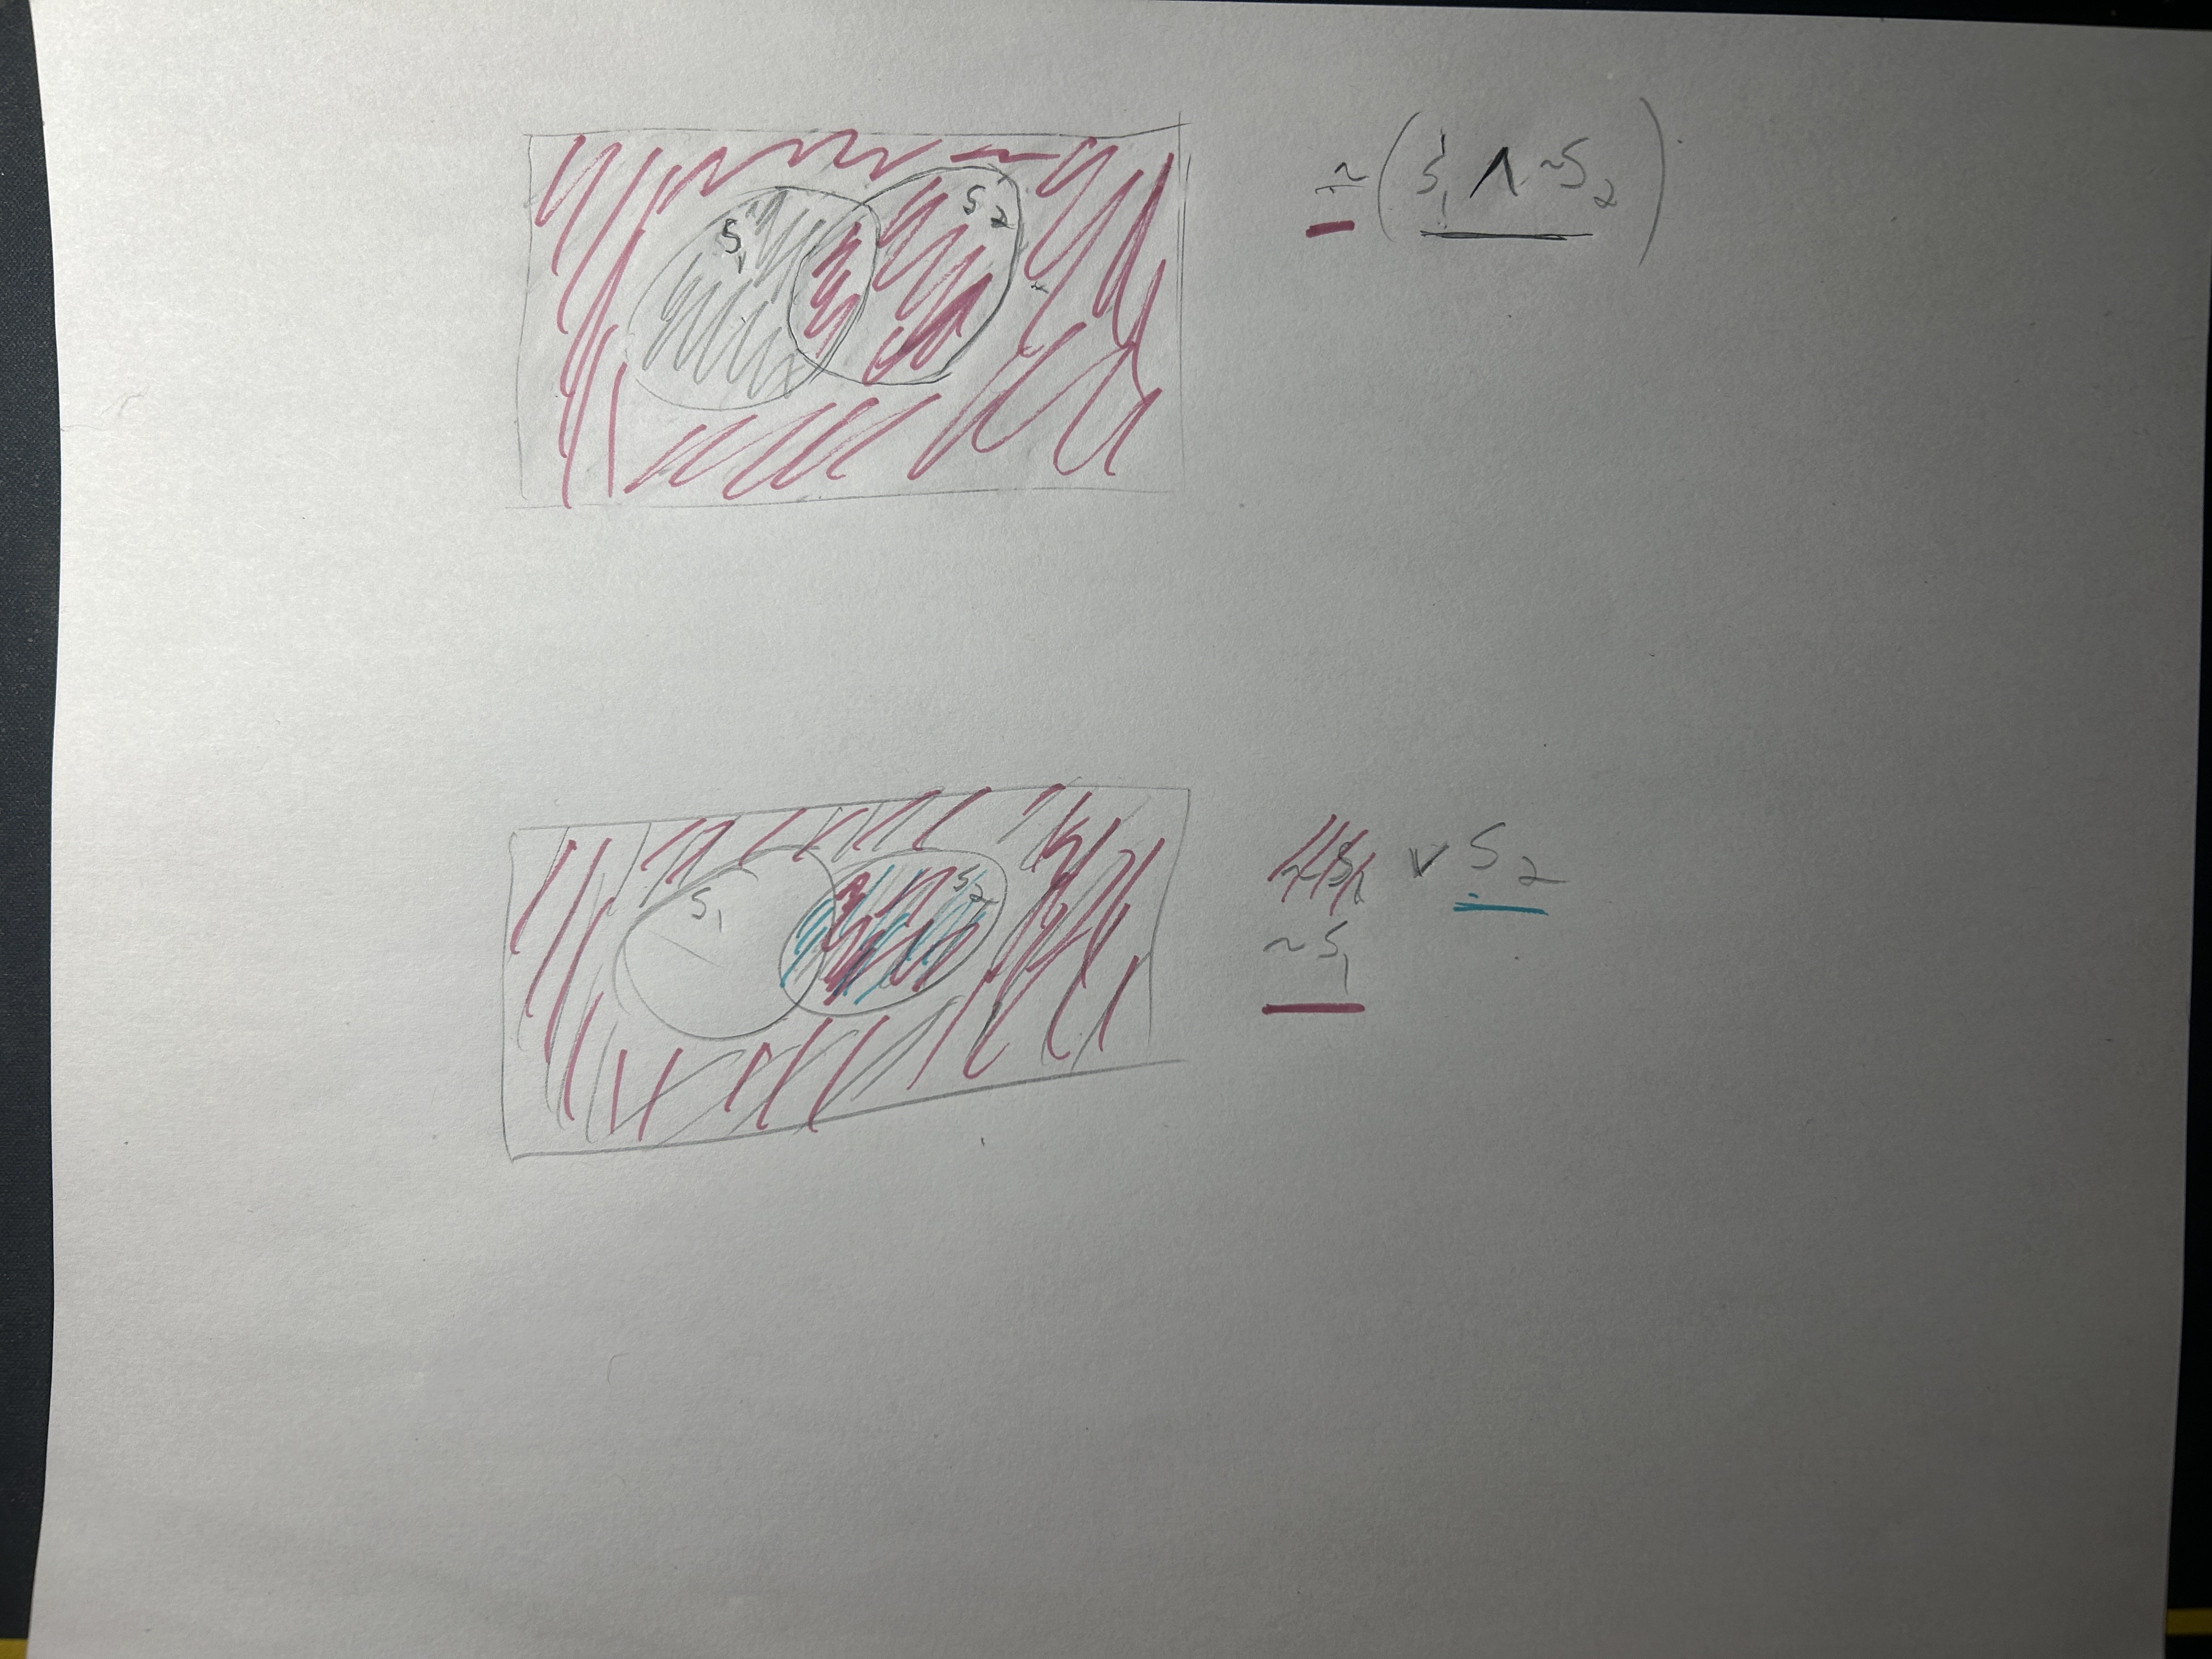
\includegraphics[scale=.1]{one.jpg} 

			\item 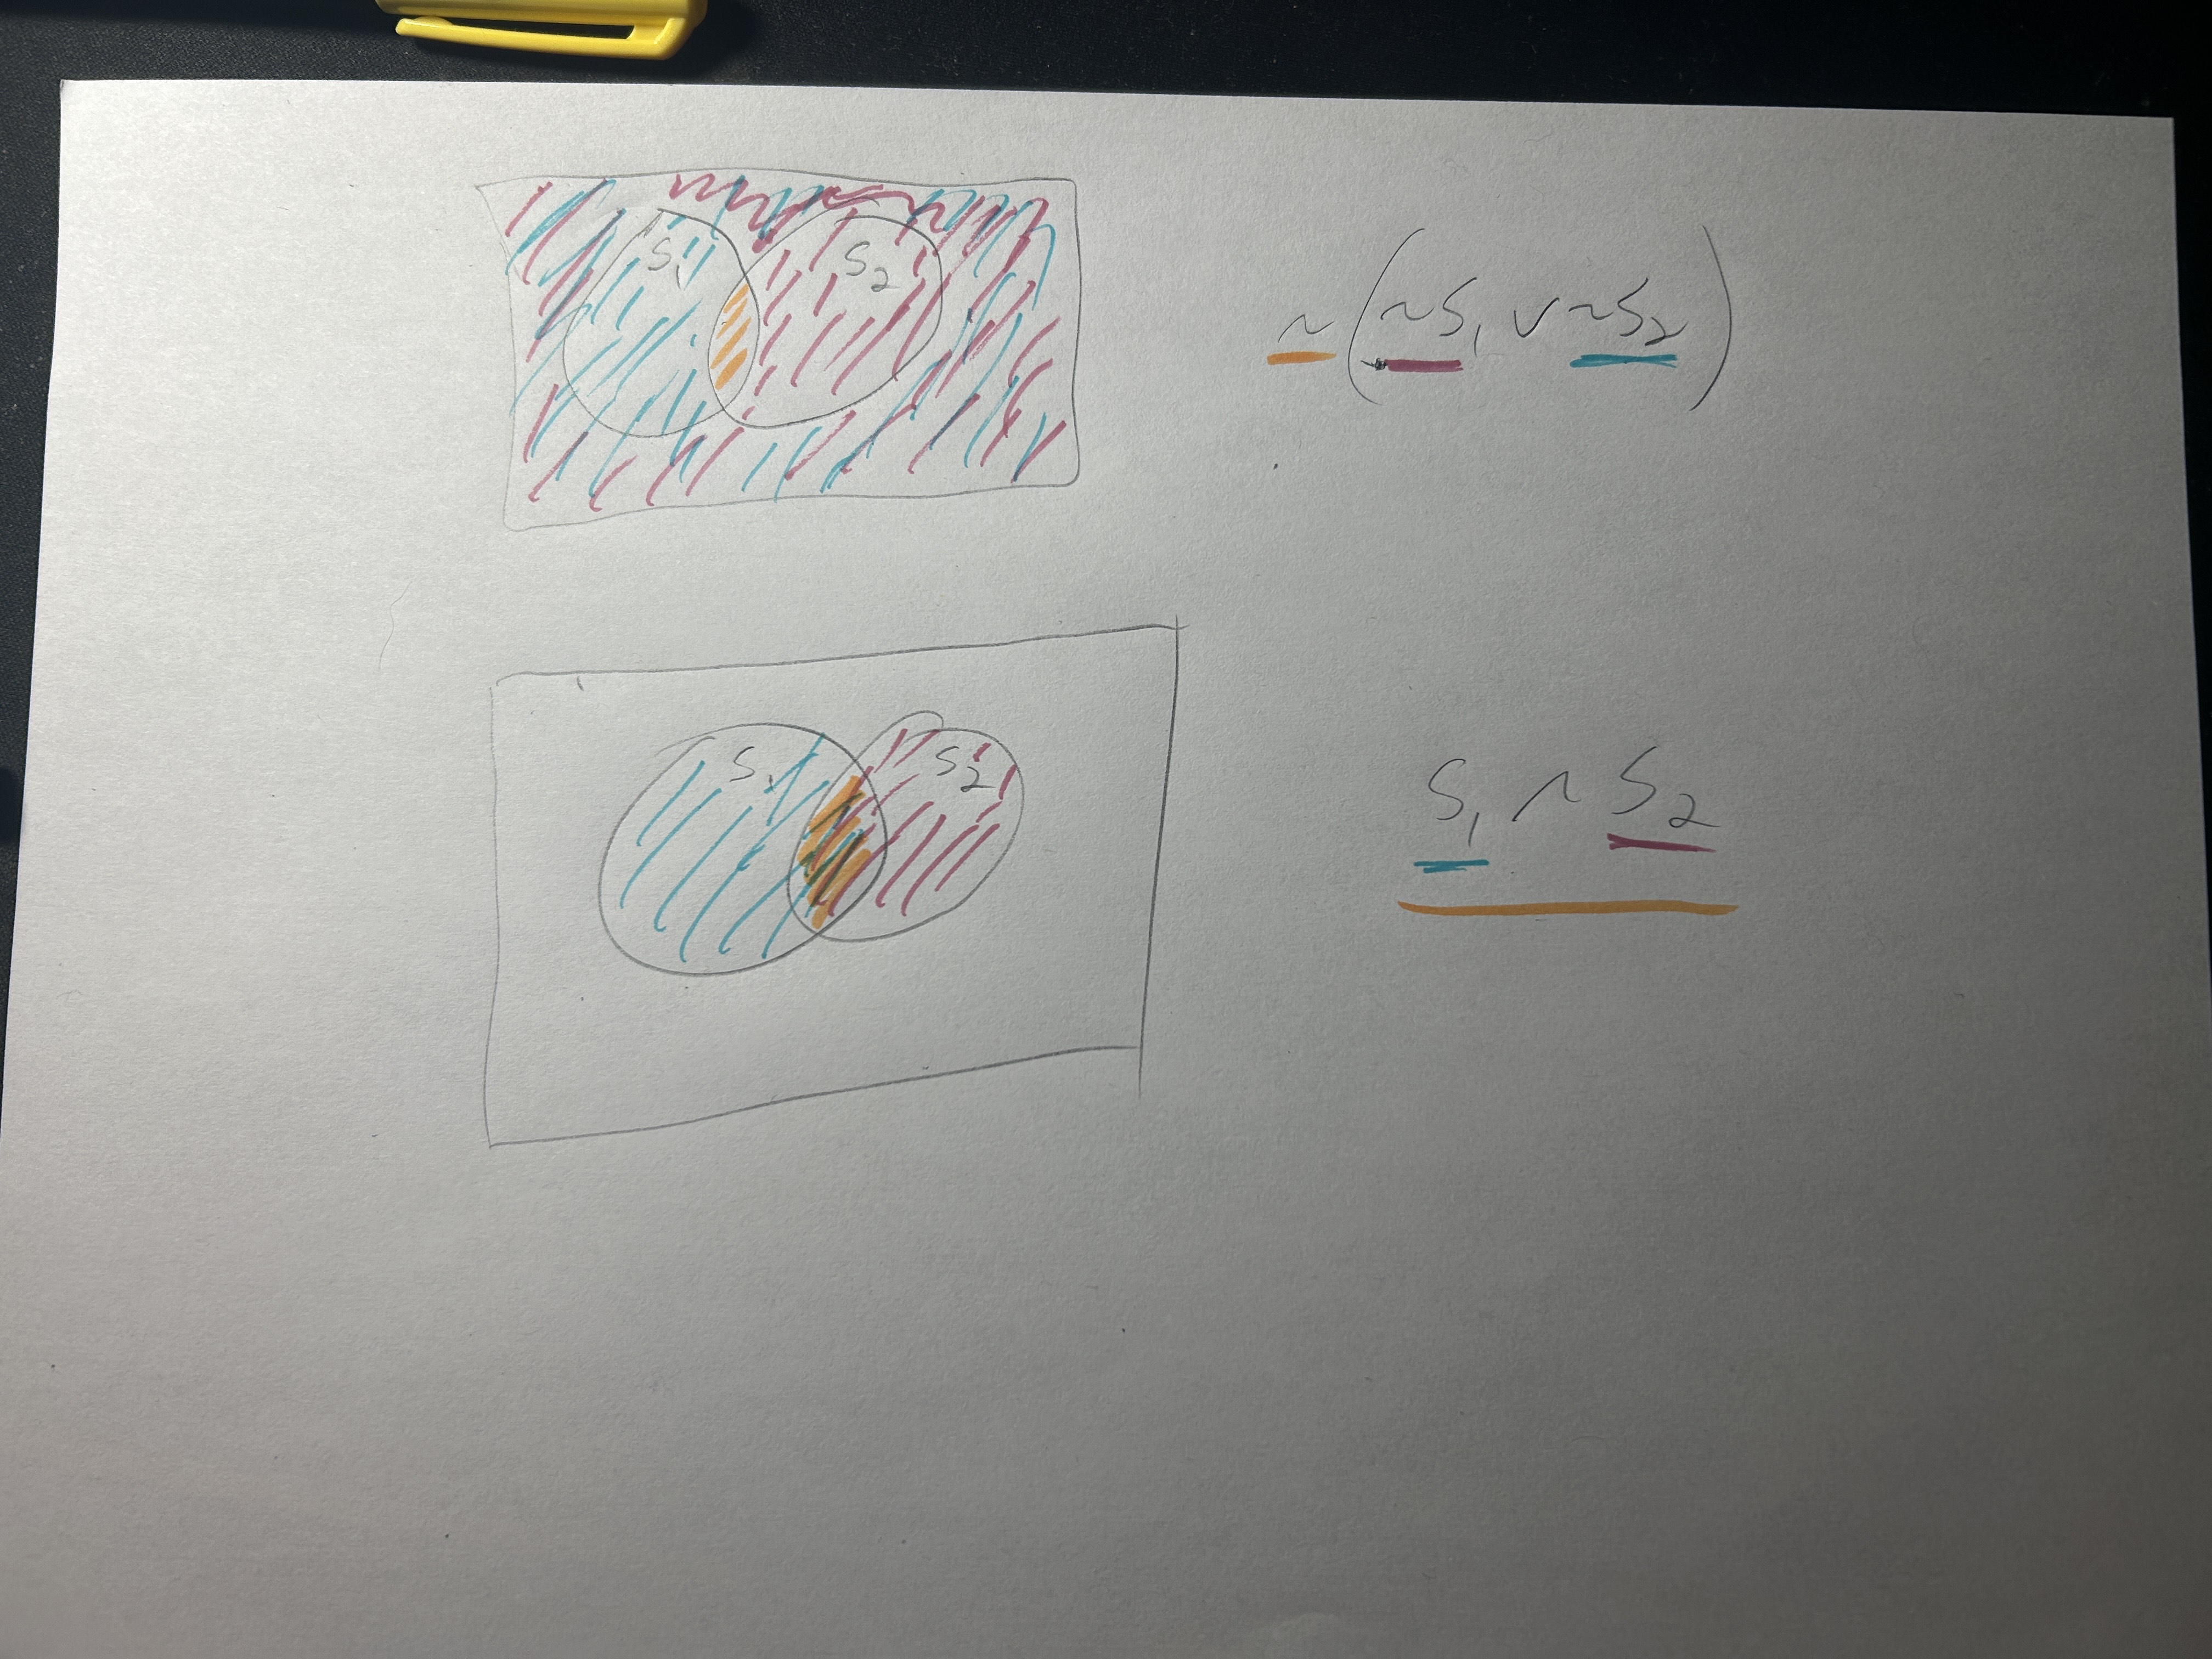
\includegraphics[scale=.1]{two.jpg}


	   	\end{enumerate}
	   \end{proof} 

	   \begin{prb}  \end{prb} 
	   \begin{proof} 
	   	Suppose not, then fix $x \in \R$ such that $x$ is irrational, but $x + 3 \in \Q$. Then there 
		exits $a, b \in \Q$ such that $x+3 = \frac{a}{b}$, then subtracting $3$ from both sides gives 
		\[ x = \frac{a}{b} - 3 = \frac{a}{b} - \frac{3b}{b} = \frac{a-3b}{b} \] 
		but since $\Z$ is closed under multiplication and subtraction, $a - 3b \in \Z$, that is, 
		we have written $x$ as a ratio of two integers, contradicting our assumption that $x$ is irrational. 
	   \end{proof} 

	   \begin{prb}  for $n \in \N$, $n^2 -3n + 9\geq 0$. \end{prb} 
	   \begin{proof} 
		   First, assume that $n \geq 3$, then write $n = 3 + a$ for $a \in \N \cup \{0\}$. 
		   we have 
		   \[ n^2 -3n + 9 = 9 + 3a + a^2 - 9 - a + 9 = 9 + 2a + a^2 \] 
		   but $a$ is non negative, so that $2a + a^2 \geq 0$, and the sum of two non negative numbers 
		   is non negative. 
		   On the other hand, suppose that $n < 3$, we just need to show that $-3n + 9 > 0$ since
		$n^2 > 0$ is always true. We have 
		\[ n < 3 \implies n < \frac{-9}{-3} \implies -3n > -9 \implies -3n + 9 > 0 \] 
		as desired. 
	   \end{proof} 
	

	   \begin{prb}  \end{prb} 
	   \begin{proof} 
	   	\begin{enumerate}[(a)]
	   		\item True, because any two points only appear in a single line
				\item  True, every line does contain at least two points 
				\item True, there is no line containg $A, B$ and $D$.
				\item It satisfies the Elliptic parallel property, 
					since $\{A, B, C\}$ contains every point save for $D$, 
					but every other line containing $D$ contains one of $A$, $B$, or $C$. 
					Further, if we start with a line containing $D$, then it also 
					contains $A, B$ or $C$, so that it is incident with every other line. 
				\item Yes it is since it satisfies the 3 axioms of an incidence geometry. 
	   	\end{enumerate}
	   \end{proof} 
\end{document}
